\documentclass[conference]{IEEEtran}
\IEEEoverridecommandlockouts
% The preceding line is only needed to identify funding in the first footnote. If that is unneeded, please comment it out.
\usepackage{cite}
\usepackage{amsmath,amssymb,amsfonts}
\usepackage{graphicx}
\usepackage{textcomp}
\usepackage{xcolor}
\def\BibTeX{{\rm B\kern-.05em{\sc i\kern-.025em b}\kern-.08em
    T\kern-.1667em\lower.7ex\hbox{E}\kern-.125emX}}
\title{
\vspace{1cm}
{
\includegraphics[width=0.15\textwidth]{           /storage/emulated/0/vignan/IMG-20241018-WA0001.jpg} \\ 7447 BCD - Seven segment Display Decoder Assignment} }
\author{Bynaboyina Aiswarya \\ Roll No: FWC22295 \\ aiswaryabaiswarya61@gmail.com}
 \begin{document}
\maketitle
 \section {ABSTRACT}
 This paper shows how to use the 7447 BCD-Seven segment Display Decoder to learn Boolean logic using arduino uno.

\section{COMPONENTS}
The required components list is given in Table: I. and seven segment display is shown in Fig.2 and IC 7447 diagram is shown in Fig.1.
\vspace{0.3cm}
 \begin{table} [htbp]
\centering
\begin{tabular}{| c | c | c |} \hline
Components & Value & Quantity \\\hline
IC & 7447 & 1 \\ \hline
seven segment display & & 1\\ \hline
Arduino & UNO & 1 \\ \hline
Jumper Wires &  & 10 \\ \hline
Breadboard & & 1 \\ 
\hline
\end{tabular}
\vspace{0.3cm}
\caption{\label{tab:widgets}}
\end{table}

\begin{figure}[h]                           
\centering                            
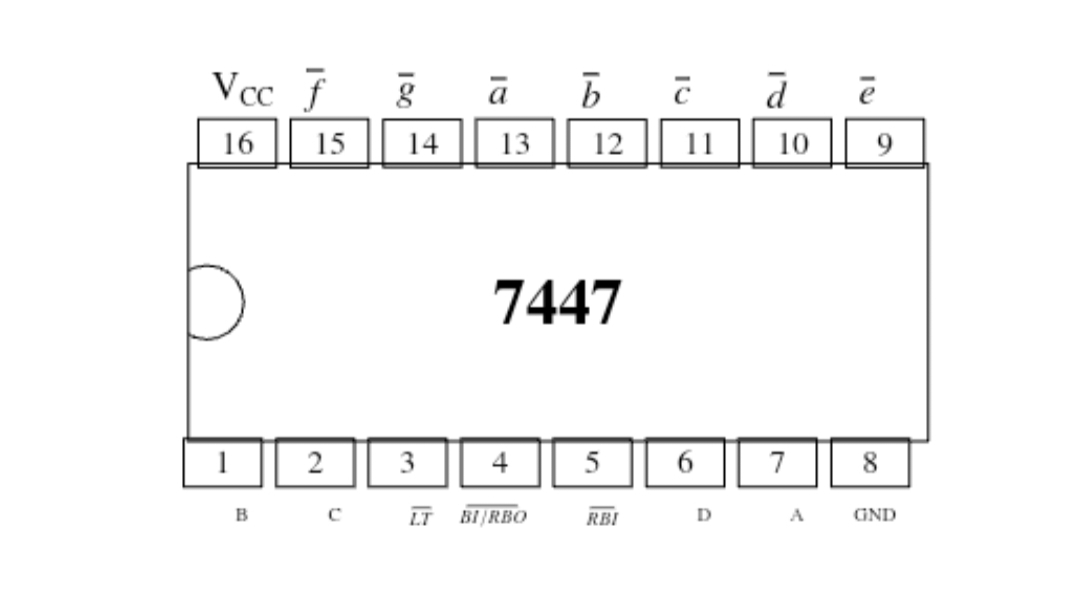
\includegraphics[width=0.5\textwidth]{ /storage/emulated/0/vignan/IMG_20241019_200414.jpg }                      
\caption{\label{fig-1:Gates}}           
\end{figure}

\begin{figure}[h]                           
\centering                                 
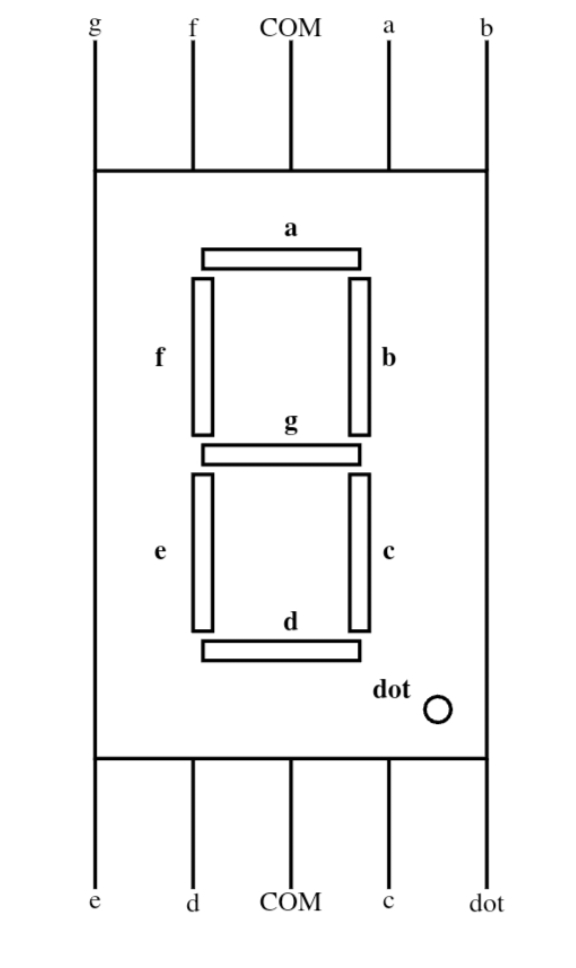
\includegraphics[width=0.3\textwidth]{ /storage/emulated/0/vignan/IMG_20241019_200944.jpg}                                           
\caption{\label{fig-2:Gates}}               
\end{figure}


\section{PROCEDURE}


\begin{enumerate}
\item Make the connections of 7447 IC and seven segment display as per below Fig.3.
	\begin{figure}[h] 
	\centering 
	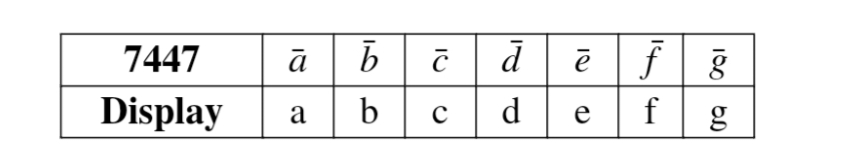
\includegraphics[width=0.3\textwidth]{ /storage/emulated/0/vignan/IMG_20241019_211433.jpg }
	\caption{\label{fig-3:Gates}}    
\end{figure}

\item Make the connections of 7447 IC and arduino uno as per below Fig.4.            
\begin{figure}[h]                     
\centering                           
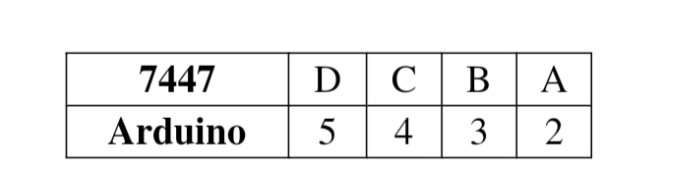
\includegraphics[width=0.3\textwidth] { /storage/emulated/0/vignan/IMG_20241019_212154.jpg    }                                 
\caption{\label{fig-4:Gates}}         
\end{figure}

\item {Truth Table for incrementing from $0$ to $9$ in seven segment display }
	\vspace{0.4cm}

\begin{table}[htbp]
    \centering
\begin{tabular}
{ | c | c | c | c | c | c | c | c | } \hline
$Z$ & $Y$ & $X$ & $W$ & $D$ & $C$ & $B$ & $A$\\\hline
0   & 0   & 0   & 0   & 0  & 0 & 0  & 1 \\
0   & 0   & 0   & 1   & 0  & 0 & 1  & 0 \\
0   & 0   & 1   & 0   & 0  & 0 & 1  & 1 \\
0   & 0   & 1   & 1   & 0  & 1 & 0  & 0 \\
0   & 1   & 0   & 0   & 0  & 1 & 0  & 1 \\  
0   & 1   & 0   & 1   & 0  & 1 & 1  & 0 \\
0   & 1   & 1   & 0   & 0  & 1 & 1  & 1 \\  
0   & 1   & 1   & 1   & 1  & 0 & 0  & 0 \\
1   & 0   & 0   & 0   & 1  & 0 & 0  & 1 \\
1   & 0   & 0   & 1   & 0  & 0 & 0  & 0 \\ \hline
\end{tabular}
\vspace{0.15cm}
\caption{\label{tab:widgets}}
\end{table}






\item Execute the arduino code without any errors.
\item After upload the code into hardware setup using arduino IDE platform with hex file.
 \end{enumerate}

\section{RESULTS}
 \begin{enumerate}
	 \item Download the code given in the link below and execute them to see the output as shown in Fig.5. 
	 \item https://github.com/BynaboyinaAiswarya/Fwc-/blob/main/Ide/7447/txt.c//
 \end{enumerate}
		 \begin{figure}[h] 
	\centering 
	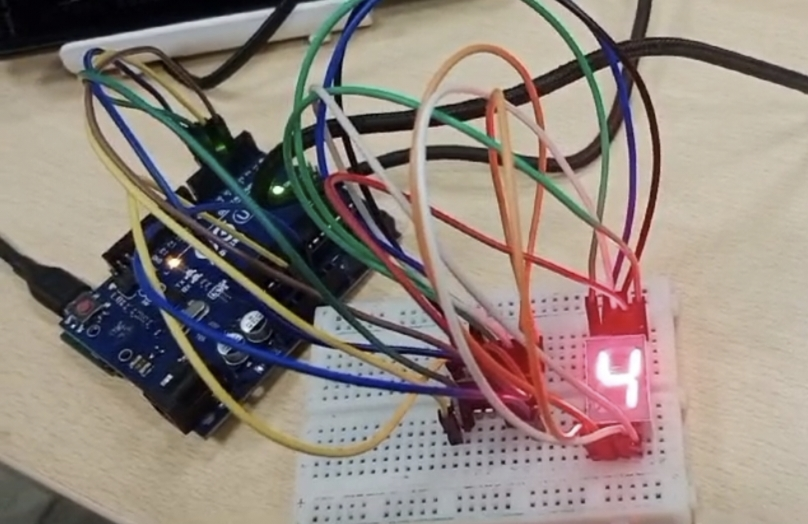
\includegraphics[width=0.4\textwidth]{  /storage/emulated/0/vignan/IMG_20241018_153316.jpg}
	\caption{\label{fig:Gates}}    
\end{figure}
\section{CONCLUSION}
Hence implementation of 7447 IC, Seven segment dispaly using arduino UNO is done.
\end{document}
